\documentclass[12pt]{upenndiss}

%bibliography
\usepackage{natbib}
\bibpunct[:]{(}{)}{,}{a}{}{,}

% phonological examples
%\usepackage{simplex}
\usepackage{amsmath}

% fonts
%\usepackage{mathspec}
%\setmainfont[Mapping=tex-text]{Linux Libertine}
%\setmathfont(Digits,Greek,Latin){Linux Libertine}
%\usepackage{microtype}
%\usepackage{coptic}


% tables and figures
\usepackage{booktabs}
\usepackage{graphicx}
\usepackage{floatrow}
\usepackage{multirow}
\usepackage{enumitem}
\newfloatcommand{capbtabbox}{table}[][\FBwidth]
\setlist{noitemsep}

% Add packages and definitions you want to use here:
\usepackage{times}
\usepackage{multirow,sectsty}
\usepackage{setspace}
\usepackage{subfigure,graphicx}
\usepackage{amsmath,amsthm,amsfonts, amssymb}
\theoremstyle{definition} \newtheorem{definition}{Definition} 
\usepackage{linguex}
% \usepackage{betababel}
\usepackage[english,greek]{betababel}
\usepackage{tikz-qtree}
\usepackage{tikz}
\usetikzlibrary{arrows,automata,chains,matrix,positioning,scopes}

\usepackage[normalem]{ulem}

\usepackage{pdfpages}

\usepackage{natbib}

\usepackage{epigraph}
\usepackage{hyperref}

 \usepackage[only, llbracket,rrbracket]{stmaryrd}
 \newcommand{\sem}[1]{\ensuremath{\{ #1 \} }}
 \newcommand{\pair}[1]{\ensuremath{\langle #1 \rangle}}
 \newcommand{\la}{\ensuremath{\lambda}}
 \newcommand{\inter}[1]{\ensuremath{\llbracket#1\rrbracket}}

\newcommand*\circled[1]{\tikz[baseline=(char.base)]{
            \node[shape=circle,draw,inner sep=2pt] (char) {#1};}}


\newcommand{\comm}[1]{}
\long\def\symbolfootnote[#1]#2{\begingroup%
\def\thefootnote{\fnsymbol{footnote}}\footnote[#1]{#2}\endgroup}

\begin{document}

\setcounter{chapter}{3}
\chapter{Cycles}
\label{Cycles}

\setlength{\epigraphwidth}{.9\textwidth}

\epigraph{[T]o say what a word means in a language is to say what
it is in general optimal for speakers of that language to
do with that word, or what use they are to make of it.\\--H.P. Grice \citeyearpar[299]{grice1989} \\ \vspace{12pt}
I can't say `It's cold here' and mean `It's warm here' -- at least, not without a little help from my friends.\\--David Lewis \citeyearpar{lewis:1969}}


Distinguishing between the formal and functional Jespersen cycles clarifies what needs to be explained. Given that the functional cycle can occur independently of the formal cycle, an explanation of the functional cycle is required even in the absence of an explanation of the formal cycle. In this chapter we develop a model of the functional cycle using the mathematical framework developed in Chapter 3. In particular, we make explicit the notion of \emph{emphasis} that captures the intuitive distinction between forms: the incoming form expresses something above and beyond the meaning of the incumbent form. 

\cite{schwenter2005,schwenter2006}, which takes the notion of emphasis to be a result of the conditioning effects of discourse and information structure. While the details of the two accounts differ, they share an abstract structure. Namely, the functional distinction between forms can be conceptualized as a scale: emphatic forms are introduced at the high end of the scale and move down it as their emphasis fades. It is their movement along this dimension that constitutes their fading.  

we describe the underlying scale that the different forms move through. We then characterize each analysis as a signaling game and determine its equilibria. Using the evolutionary game-theoretic framework developed in Chapter 3, we examine how signaling changes under the evolutionary game dynamics. Finally, we fit the two resulting models to corpus data and evaluate the fitted parameters.


%Traugott (1989) and others argue that semantic change typically proceeds gradually through polysemy and ambiguity, driven by the conventionalization of pragmatic inferences. She identifies three tendencies of semantic change based on her investigation of English modal auxiliaries (1989: 34-35):
%\begin{enumerate}
%	\item Meanings based in the external described situation $>$ meanings based in the internal (evaluative/perceptual/cognitive) described situation.
%	\item Meanings based in the external or internal described situation $>$ meanings based in the textual and metalinguistic situation.
%	\item Meanings tend to become increasingly based in the speaker's subjective belief state/attitude toward the proposition.
%\end{enumerate}



%Both the first and the last of these equilibria are pooling equilibria. That is, senders only ever use a single signal. In response to this, receivers take the action that maximizes their expected utility given the prior probability distribution over types. That is, they guess the expected value of the type space. They simply infer the average standard of precision.
%
%In contrast, the middle equilibrium constitutes a partially separating equilibrium. It is only partially separating because the state space is infinite, while the message space is not. This means that every type cannot be fully revealed, but that some information is transferred. The amount of information transferred and the distinction between the partially separating and pooling equilibria can be characterized in information-theoretic terms \citep{shannon:1948}. In particular, we can think of the amount of information conveyed by a particular signal at equilibrium according to the \emph{Kullback-Leibler Divergence} \citeyearpar{kullback-leibler1951divergence}.
%
%\begin{equation}
%     D_{KL}(P || Q) = \int_{-\infty}^{\infty} log\left( \frac{p(x)}{q(x)}  \right)p(x) dx
%\end{equation}
%This serves as a measure for how much change is induced in the receiver by a particular message. That is, in our case $q(x)$ corresponds to the prior probability distribution over types, and $p(x)$ corresponds to the probability of a sender being of a particular type given the message. The more the message shifts the probability from the prior, the more information it conveys. And, the less a message shifts the probability from the prior, the less information it conveys. 
%


%We have established an upper limit on the amount of bias that allows for two signals to be used informatively. If this bias is exceeded, then signaling collapses. A single message is used, but carries no information. In fact, for a given number of signals, $n$, there exists some level of bias, $b_n$, that allows for their informative use in a partially separating equilibrium based on a sender's partition of the type space, $\mathcal{P}_n$ \citep{crawford-sobel:1982}. As the number of signals increase, the amount of bias must decrease to allow for informativity, thus $b_2 > b_3 > ... > b_n$. Intuitively, as the preferences of senders and receivers approach each other a finer and finer partition of the space is possible.

%\subsection{Dynamics}

%So, what does this mean for Jespersen's cycle? Intuitively, the pragmatics of emphasis suggest that the population originally starts at a point where one form is used with a  very high standard of precision and another is used for all other standards. That is, emphatic negation is distinguished from plain negation in its contexts of use. We can determine what will happen to these two signals over time. Intuitively, under the game dynamics, the signals will converge to their equilibrium use.
%
%Under the game dynamics, for any amount of bias, no matter how slight, the emphatic form will spread to lower and lower standards of precision until it reaches its equilibrium use. The amount of bias determines where this process stops. That is, if a partially separating equilibrium exists, then the emphatic form will expand to encompass all standards of the upper part of the partition. In other words, the emphatic will be \emph{attenuated}, but still carry some information.  If no separation is possible, the emphatic form will spread across all standards. In other words, the emphatic will be entirely \emph{bleached} of its emphasis. Note that in both cases the process can be characterized in information-theoretic terms. That is, as the emphatic form spreads to more and more standard it conveys less and less information. 
%
%The stable coexistence of plain and emphatic negation for long periods of time suggest that the bias is sufficiently small to allow for at least two forms. This, however, raises the question of what destabilizes the system. The system must be disturbed by a push chain, whereby the signal used for the lowest subinterval is lost. More generally, imagine a system with bias $b_n$ at equilibrium. Now, suppose that a new signal is introduced, so that there are now $n+1$ signals. Clearly, the system is not stable. However, it will be carried back to some equilibrium by the game dynamics. The resultant equilibrium depends on the character of the signal that is introduced. Let $a'$ be the response of receivers to the new signal $m'$. All messages that receive a lower response than $a'$ will be pushed down, the lowest of these being pushed out of use completely.  In the case of Jespersen's Cycle, new signals enter with a high $a'$, and thus displace everything below. That is, they are emphatic and lead hearers to 
%infer a high standard of precision. This means that all other forms lower in the scale will be pushed down and the lowest will be pushed out of existence, exactly like what we see in the actual instantiation of the cycle.


\section{Discourse Status}

\cite{schwenter2005,schwenter2006} uses synchronic data from several Romance languages to show that the notion of emphasis as it relates to the functional cycle may better explained by discourse conditions. In particular, he shows that different forms of negation are sensitive to information structure, most notably, the discourse status of the proposition being negated. While Schwenter's analysis relies on synchronic data, \cite{hansen2009, hansen-visconti2009,hansen-visconti2012} have used historical corpora of French and Italian to show similar conditioning of the embracing form. 

% \cite{hansen2009, hansen-visconti2009,hansen-visconti2012} have used historical corpora of French and Italian to show that the embracing form (\textsc{\color{blue} neg V neg}) is sensitive to the discourse status of the proposition being negated. Namely, the embracing form is restricted to instances where the proposition being negated is either \textsc{discourse old} or \textsc{inferrable}.
%That is, \emph{\textsc{\color{blue} neg V neg}} is sensitive to the discourse status of the proposition being negated.

In what follows, we use examples from Brazilian Portuguese which exhibits pre-verbal \textsc{\textcolor{red}{neg V}}, embracing  \textsc{\color{blue} neg V neg}, and post-verbal forms \textsc{\color{green} V neg}, to demonstrate the sensitivity of negation to these distinctions. Before doing so, however, we should note that these forms are unique in the sense that they are all realized as the negator \emph{n{\~a}o}.  Thus, this may be a unique case where both transitions in the formal cycle contain functional cycles.

To begin, consider the following scenario. Suppose that a husband and wife expect a plumber to come fix their leaky faucet while they are at work during the day. The husband arrives home before his wife to find a still leaky faucet. The wife arrives home shortly and the first thing her husband says is the following.



\exg.  O bombeiro \textcolor{red}{ n{\~a}o} \textcolor{red}{veio}.\\
         The plumber NEG came\\
         ``The plumber didn't come."\\

\exg. \#O bombeiro \textcolor{blue}{n{\~a}o} \textcolor{blue}{veio} \textcolor{blue}{n{\~a}o}.\\
	The plumber NEG came NEG\\
	``The plumber didn't come."\\

The reason that the embracing form is odd is that it comes out of the blue, so to speak. That is, the proposition ``The plumber came.'' is entirely \emph{discourse new} in the sense of \cite{prince:1992}. In this case, the \emph{discourse} is the set of entities and propositions that have been introduced during a conversation.  Even if the husband has some expectation that his wife has been thinking about whether or not the plumber came, the proposition has not been introduced into the discourse yet. The first condition on the forms of negation is that the embracing form cannot be used to negate \emph{discourse new} propositions.

However, a proposition can be introduced into the discourse in several ways, both explicitly and implicitly. For example, if the wife walks in the door asks the following.

\exg.  O bombeiro veio hoje?\\
       The plumber came today\\
         ``Did the plumber come today?"\\

Asking the question has explicitly introduced the proposition into the discourse, making either form appropriate in the husband's response. In fact, the wife need not even explicitly ask the question. For example, if she arrives home and points quizzically at the sink, then the embracing form is felicitous. This is because the proposition can be inferred from the discourse.

Schwenter shows that even finer distinctions can be made in the sensitivity of different forms of negation to discourse context. He demonstrates two further conditions on the use of the different negative forms. For example, consider the following scenario. Suppose that two colleagues meet in a departmental hallway in the afternoon after a scheduled talk, and one asks the other the following question.

\exg. Voc{\^e} gostou da palestra da Maria?\\
	 you liked the talk of Maria\\
	 ``Did you like Maria's talk?"

\exg. \textcolor{blue}{N{\~a}o} \textcolor{blue}{fui} \textcolor{blue}{n{\~a}o}.\\
	 NEG went NEG\\
	 ``I didn't go."\\

\exg. \#\textsc{\color{green}Fui} \textsc{\color{green}n{\~a}o}.\\
	  went neg\\
	 ``I didn't go."\\

The reason that the post-verbal form is odd is that the proposition being negated ``I went (to Maria's talk).'' is only indirectly connected to the discourse. That is, liking a talk presumably requires having attended it, so the proposition is only \emph{inferrable} from the discourse. The post-verbal form can only be used where the proposition is discourse old. This is made clear by altering the form of the response to the question of liking the talk.

\exg. \textsc{\color{blue}N{\~a}o} \textsc{\color{blue}Gostei} \textsc{\color{blue}n{\~a}o}.\\
	 neg liked neg\\
	 ``I didn't like it."\\

\exg. \textsc{\color{green}Gostei} \textsc{\color{green}n{\~a}o}.\\
	  liked neg\\
	 ``I didn't like it."\\

In this case the post-verbal form is acceptable because the proposition ``I liked Maria's talk.'' has been introduced into the discourse by the original question. The conditions and restrictions on different forms can be summarized as in Table \ref{schwenter}. The pre-verbal form is acceptable in any context, but the other two forms are only acceptable in more and more restricted contexts,

\begin{table}
\begin{center}
\begin{tabular}{@{}ccccc@{}}
      \hline
       & \textsc{discourse new} & \textsc{inferrable} & \textsc{discourse old}\\ \hline
      \textsc{\color{red} neg V} & $\checkmark$ &  $\checkmark$ &  $\checkmark$ \\
      \textsc{\color{blue} neg V neg} & \#  & $\checkmark$ & $\checkmark$ \\
      \textsc{\color{green} V neg} & \#  & \#  & $\checkmark$ \\
      \hline
\end{tabular}     
\end{center}
\caption{Acceptability of forms in discourse contexts}     
\label{schwenter}
\end{table}

It is not entirely clear if the forms of negation in Brazilian Portuguese should be treated differently than the canonical case of the formal cycle as in English and French. However, languages with only the pre-verbal and embracing form exhibit the same sensitivity to discourse status (e.g. \cite{schwenter2006} for Catalan and Italian, \cite{hansen2009} for French). Namely, languages that only have two forms make the distinction between \emph{discourse new} and everything else. That is, The embracing form is available in discourse old and inferable contexts, but not discourse new contexts, whereas the pre-verbal form is allowed in all contexts.  

%This, of course raises the question of whether the post-verbal form is necessarily sensitive to discourse status or is the result of other processes, such as phonetic reduction. These are open empirical questions, which might also vary by the particular circumstances of a language.

The shape of the conditioning factors suggests an intuitive characterization. That is, the different forms of negation are sensitive to the scale of how closely the negated proposition is connected to the discourse. That is, if we take connection to the discourse as a continuous measure, then discourse new propositions are at the low end, discourse old propositions are at the high end, and inferable propositions are somewhere in the middle. In fact, we can simply reduce this to a scale of degrees of inferability: discourse new propositions are not inferable since we cannot read minds, and discourse old propositions are completely inferable since they have just been explicitly introduced into the discourse. 

At the beginning of the functional cycle the incoming form is restricted to a smaller range of contexts. In the case of English, among others, it is restricted to those contexts where the proposition being negated has just been mentioned or introduced into the discourse. Subsequently, the embracing form increases in frequency and is used in more and  more contexts. As it is used in more and more contexts it loses its specialized meaning. At the end point of the functional cycle, where the embracing form is used across all contexts, it ceases to carry any specialized meaning. Note that this is entirely parallel to the trajectory described above for standards of precision. Thus, the functional cycle can be conceived of as of one form taking the place of another along a continuous semantic dimension.


The motivation of this project stems from particular hypotheses about the conditioning factors of negation in Jespersen's Cycle \citeyearpar{jespersen:1917}, which can be characterized by the transition from pre-verbal to embracing to post-verbal negation: \textsc{\color{red} neg V} $\rightarrow$ \textsc{\color{blue} neg V neg} $\rightarrow$ \textsc{\color{green} V neg}. In particular, \cite{hansen2009, hansen-visconti2009,hansen-visconti2012} have used historical corpora of French and Italian to show that the embracing form (\textsc{\color{blue} neg V neg}) is sensitive to the discourse status of the proposition being negated. Namely, the embracing form is restricted to instances where the proposition being negated is either \textsc{discourse old} or \textsc{inferrable}.

\cite{schwenter2005,schwenter2006} uses synchronic data from Brazilian Portuguese to demonstrate the sensitivity of negation to these distinctions. Consider the following scenario. Suppose that a husband and wife expect a plumber to come fix their leaky faucet while they are at work during the day. The husband arrives home before his wife to find a still leaky faucet. The wife arrives home shortly and the first thing her husband says is the following.

\exg.  O bombeiro \textsc{\color{red} n{\~a}o} \textsc{\color{red} Veio}.\\
         The plumber neg came\\
         ``The plumber didn't come."\\

\exg. \#O bombeiro \textsc{\color{blue}n{\~a}o} \textsc{\color{blue}Veio} \textsc{\color{blue}n{\~a}o}.\\
	The plumber neg came neg\\
	``The plumber didn't come."\\

The reason that the embracing form is odd is that it comes out of the blue, so to speak. That is, the proposition ``The plumber came.'' is entirely \textsc{discourse new}. Even if the husband has some expectation that his wife has been thinking about whether or not the plumber came, the proposition has not been introduced into the \emph{discourse} yet. The embracing form cannot be used to negate \textsc{discourse new} propositions.

However, how the proposition can be introduced into the discourse in several ways, both explicitly and implicitly. For example, if the wife walks in the door and says the following.

\exg.  O bombeiro veio hoje?\\
       The plumber came today\\
         ``Did the plumber come today?"\\

Asking the question has explicitly introduced the proposition into the discourse, making either form appropriate in the husband's response. In fact, the wife need not even explicitly ask the question. For example, if she arrives home and points quizzically at sink, then the embracing form is fine. This is because the proposition can be inferred from the discourse.

Schwenter shows that even finer distinctions can be made in the sensitivity of different forms of negation to discourse context. For example, consider the following scenario. Suppose that two colleagues meet in a departmental hallway in the afternoon after a scheduled talk, and one asks the other the following question.

\exg. Voc{\^e} gostou da palestra da Maria?\\
	 you liked the talk of Maria\\
	 ``Did you like Maria's talk?"

\exg. \textsc{\color{blue}N{\~a}o} \textsc{\color{blue}Fui} \textsc{\color{blue}n{\~a}o}.\\
	 neg went neg\\
	 ``I didn't go."\\

\exg. \#\textsc{\color{green}Fui} \textsc{\color{green}n{\~a}o}.\\
	  went neg\\
	 ``I didn't go."\\

The reason that the post-verbal form is odd is that the proposition being negated ``I went (to Maria's talk).'' is only indirectly connected to the discourse. That is, liking a talk presumably requires having attended it, so the proposition is only \textsc{inferrable} from the discourse. The post-verbal form cannot be used where the proposition is discourse new or inferrable. This is made clear by altering the form of the response to the question of liking the talk.

\exg. \textsc{\color{blue}N{\~a}o} \textsc{\color{blue}Gostei} \textsc{\color{blue}n{\~a}o}.\\
	 neg liked neg\\
	 ``I didn't like it."\\

\exg. \textsc{\color{green}Gostei} \textsc{\color{green}n{\~a}o}.\\
	  liked neg\\
	 ``I didn't like it."\\

In this case the post-verbal form is acceptable because the proposition ``I liked Maria's talk.'' has been introduced into the discourse by the original question. The conditions and restrictions on different forms can be summarized as in Table \ref{schwenter}. The pre-verbal form is acceptable in any context, but the other two forms are only acceptable in more and more restricted contexts,

\begin{table}
\begin{center}
\begin{tabular}{@{}ccccc@{}}
      \hline
       & \textsc{discourse new} & \textsc{inferrable} & \textsc{discourse old}\\ \hline
      \textsc{\color{red} neg V} & $\checkmark$ &  $\checkmark$ &  $\checkmark$ \\
      \textsc{\color{blue} neg V neg} & \#  & $\checkmark$ & $\checkmark$ \\
      \textsc{\color{green} V neg} & \#  & \#  & $\checkmark$ \\
      \hline
\end{tabular}     
\end{center}
\caption{Acceptability of forms in discourse contexts}     
\label{schwenter}
\end{table}


It is not entirely clear if the forms of negation in Brazilian Portuguese should be treated differently than the canonical cases of embracing negation in Jespersen's Cycle (cf. \emph{ne...pas} in French, \emph{ne...not} in English). However, languages with only the pre-verbal and embracing form have been shown to exhibit this same sensitivity to discourse status (e.g. \cite{schwenter2006} for Catalan and Italian, \cite{hansen2009} for French). Namely, languages that only have two forms make the distinction between \textsc{discourse new} and everything else. This, of course raises the question of whether the post-verbal form is necessarily sensitive to discourse status or is the result of other processes, such as phonetic reduction. These are open empirical questions, which might also vary by the particular circumstances of a language.

However, the general shape of the conditioning factors suggests an intuitive characterization Jespersen's Cycle. That is, the different forms of negation are sensitive to the scale of how closely the negated proposition is connected to the discourse. That is, if we take connection to the discourse as a continuous measure, then discourse new propositions are at the low end, discourse old propositions are at the high end, and inferrable propositions are somewhere in the middle. In fact, we can simply reduce this to a scale of degrees of inferrability: discourse new propositions are not inferrable since we can't read minds, and discourse old propositions are completely inferrable since they have just been explicitly introduced into the discourse. 

We can represent this visually as in Figure \ref{continuum}, where we have simply taken the discrete categories used to construct Table \ref{schwenter} and treated them as a continuum. In fact, this wording is potentially misleading. If discourse status is about beliefs, then the underlying phenomenon is essentially gradient in nature. The discrete categories are useful because they correspond to portions of the continuum. While we have robust intuitions about the discrete categories, the varying strength of these intuitions suggests that the underlying phenomenon is essentially gradient in nature.

The continuous representation also offers us some insight into \emph{why} Jespersen's Cycle occurs. The reasoning is as follows. First, keeping track of what is actually part of the discourse is difficult. In fact, this is the problem of \emph{common knowledge}\footnote{In epistemic logic \emph{mutual knowledge} only requires that everyone know that $p$, without any further steps. Thus anything that is common knowledge is also mutual knowledge, but not \emph{vice versa}. \cite{lewis:1969} introduced common knowledge in Philosophy. \cite{clark-marshall1981} use the term ``mutual knowledge'' to refer to common knowledge.}, that everyone knows that $p$, that everyone knows that everyone knows that $p$, \emph{ad infinitum}. \cite{clark-marshall1981} outline a set of reasonable heuristics for circumventing this infinite regress, including physical or linguistic co-presence and community membership. While these heuristics are made with reference to resolving the problem of common knowledge, they extend equally to 
propositions. Namely, propositions can be introduced to the discourse either explicitly (linguistic co-presence) or implicitly (physical co-presence, community membership).

Second, we have ample experimental evidence that speakers have particular biases in communication. Speakers tend to overestimate how successful they are at communication. \cite{savitsky-etal:2011} had two pairs of friends participate in a simple communication task. All four participants sat back to back and were individually given lists of four-way ambiguous sentences to read out loud with a specified meaning. For example, the sentence ``It's getting hot in here.'' could be interpreted as an indirect request to open the window or an amorous advance. Participants were asked to do two things. They were asked to guess the intended meaning of the sentences spoken by the other participants. They were also asked to estimate how many of the sentences the friend they came with had guessed correctly, and how many sentences the strangers from the other pair had guessed correctly. 

The results can be seen in Figure \ref{savitsky}. Listeners were reliably above chance at guessing the intended meaning out of the four potential meanings, but, friends and strangers did not differ significantly. However, speakers had much higher expectations  for listeners, significantly overestimating how many sentences listeners would accurately guess. This suggests that, as speakers, we often tend to overestimate how transparent our utterances actually are to our listeners.


%\begin{figure}
%\begin{center}
%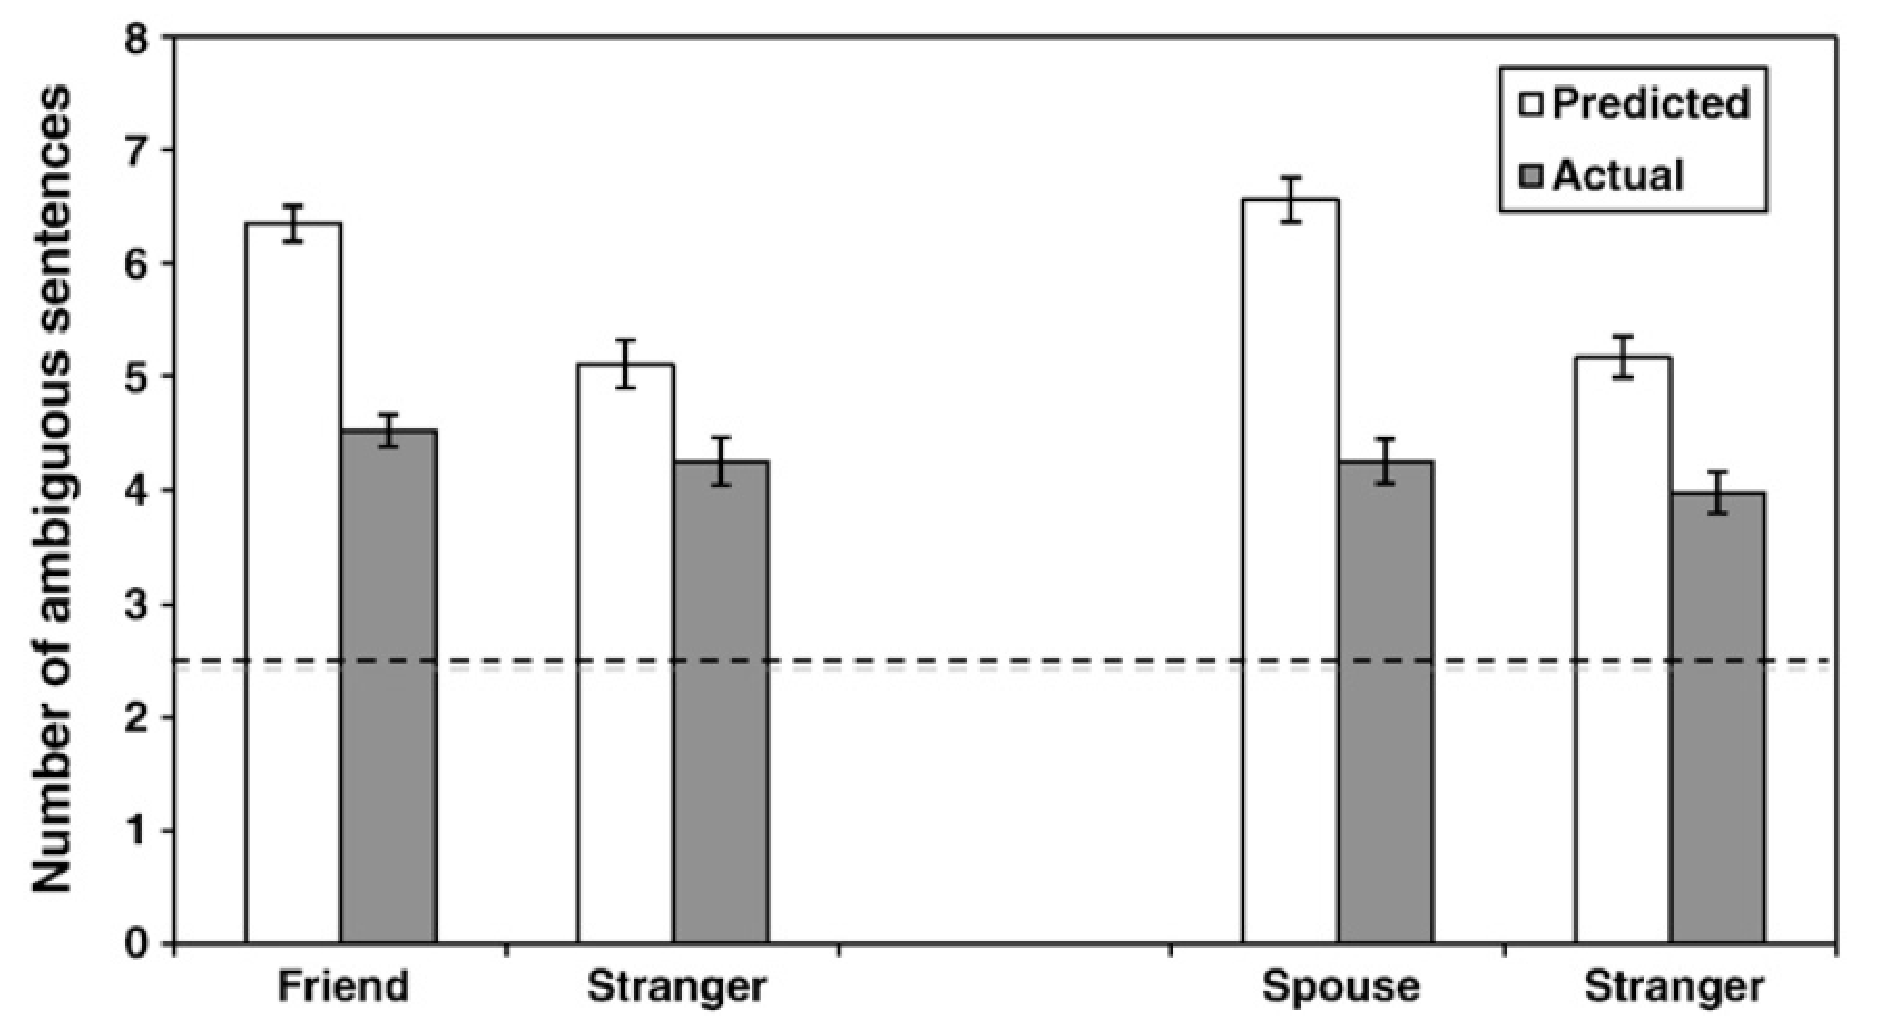
\includegraphics[width=.7\textwidth]{savitsky.pdf}          
%\end{center}
%  \caption{Results from \cite{savitsky-etal:2011}}
%   \label{savitsky}
%\end{figure}


\cite{lane-etal2006} offer evidence that is particular germane to the question of discourse status. The experimental design can be seen in Figure \ref{elephants-exp}. Participants were assigned the role of either the speaker or addressee in a communication game. Speakers were instructed to communicate information about a target shape to the addressee. One shape was visible to only the speaker, blocked from the view of the addressee by an occluder. In the target conditions, the item that was visible only to the speaker was the same shape, but varied along some relevant dimension (e.g. size, color). Figure \ref{elephants-results} shows the proportion of trials where speakers used a modifier in referring to the target item. Surprisingly, speakers' privileged information leaks into what is said. In fact, this happens to an even greater extent when speakers were explicitly instructed to conceal information about their privileged information.


%\begin{figure}
%\begin{center}
%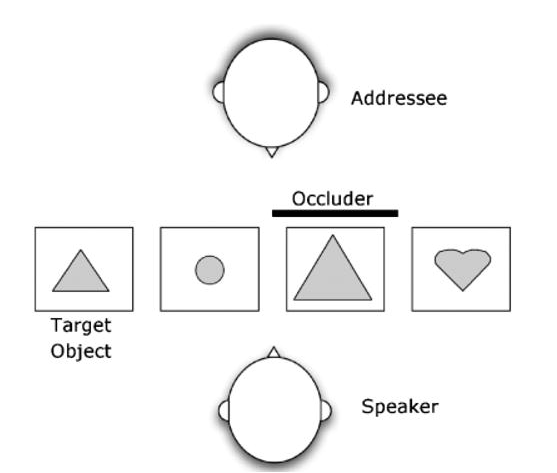
\includegraphics[width=.7\textwidth]{elephants-exp.png}          
%\end{center}
%  \caption{Experimental design of \cite{lane-etal2006}}
%   \label{elephants-exp}
%\end{figure}


%\begin{figure}
%\begin{center}
%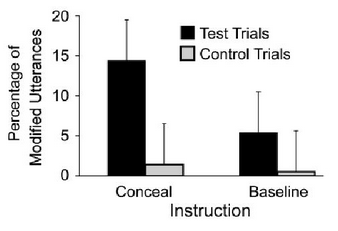
\includegraphics[width=.7\textwidth]{elephant-results.png}          
%\end{center}
%  \caption{Results for \cite{lane-etal2006}}
%   \label{elephants-results}
%\end{figure}

%Returning to Jespersen's Cycle, we note that these experimental findings suggest a potential explanation for \emph{why} change takes place. The embracing form is restricted to a particular set of contexts where the proposition being negated is discourse old, or highly inferrable. If speakers tend to overestimate how inferrable the proposition being negated is, if they fail to filter out their own privileged information, then they will tend to use the embracing form in less and less inferrable contexts. The result will be an increase in the frequency of the embracing form over time. \cite{ahern-clark2015} offer a formal model of the dynamics of this process. However, the predictions of the model, like the corpus work by \cite{hansen2009, hansen-visconti2009}, are largely qualitative. That is, they demonstrate that the different forms of negation are sensitive to different constraints at different points in time, and offer an explanation of why those constraints might change over time. However, they offer no quantitative predictions about the shape of the change.


\section{Signaling Game}


As the functional cycle proceeds, the incoming form ceases to pick out the end point of the scale. In the case of English, as the embracing form becomes more and more frequent, it ceases to signal a high standard of precision. Eventually, when the post-verbal element is obligatory, the embracing form can only convey some default standard of precision. This means that emphasis is lost. 


$S : [0,1] \rightarrow M$ 

$R : M \rightarrow [0,1]$

% $ = 0 < ... < t_{n-1} < ... < 1$ 

%\mathcal{P}_


\begin{equation}
     U_S(t, a) = 1 - (a - t - (1-t)b)^2
\end{equation}

The parameter $b$ measure the difference between the preferences of senders and receivers. To see this note that sender utility function is maximized when $a = t + (1-t)b$. When $b=0$, this means that senders prefer that the state and action correspond to each other. But, as $b$ grows, senders prefer a slightly higher action. In the extreme, when $b=1$, senders categorically prefer the action $a=1$.

In contrast, the receiver utility function is given by the following. 

\begin{equation}
     U_R(t, a) = 1 - (a - t)^2
\end{equation}

Unlike the sender utility function, the receiver utility function is maximized when the action taken by the receiver is equivalent to the sender's state. When the receiver's action matches the sender state, the second part of the function is zero, and thus the function is maximized.

%To begin, we must first consider how signaling games capture the use of negation. As we noted above, the difference between plain and emphatic negation is captured by the standard of precision applied. The speaker has knowledge about some state of the world which renders a particular negative expression acceptable on some standards, but not necessarily on others. Thus, there exists a continuum of states for the speaker, which we will take to be the interval $T = [0,1]$. The lowest possible value on such an interval corresponds to the weakest possible standard of precision that would still render the negative expression acceptable.\footnote{Here we leave out the possibility of the use of a given expression in the absence of any standard of precision being met. That is, we leave out cases of outright lying. Such cases are particularly interesting, but we leave them as a consideration for future study.} The highest possible value on the interval is then the strictest possible standard of 
%interpretation available. 
%
%Given that the speaker has observed some state of affairs, $t \in T$, he must choose a message, $m \in M$, to send to the hearer. Let $\mathcal{P}_n(T)= 0 < ... < t_{n-1} < ... < 1$ be a partition of the state space into $n$ subintervals.  A speaker's strategy is then a function from a partition of the type space to messages, $S : [\mathcal{P}_n(T) \rightarrow M]$. Intuitively, this is simply a way of carving up the state space into discrete regions and using those regions to determine which signal to send. For example, the trivial partition, $\mathcal{P}_1(T)$, occurs when the sender pools all types together and uses only a single message. In what follows we will largely be concerned with partitions of at least size two $\mathcal{P}_2(T)$. For example, consider the case of two messages, consisting of just a plain and an emphatic form. Letting $\mathcal{P}_2(T) = 0 < t_1 < 1$, a possible sender strategy is then  $s(t) = m_1$ for $t \in (0,t_1)$, and $s(t) = m_2$ for $t \in (t_1,1)$. That is, the sender uses 
%$m_1$ for all types in the first subinterval, and $m_2$ for the second subinterval. Intuitively, we would refer to $m_1$ as the plain form of negation and $m_2$ as the emphatic.
%
%Once the speaker has sent a message, the hearer is faced with the problem of how to interpret it. Given that the hearer cannot read the speaker's mind, she must infer the state of affairs that prompted the use of a particular form. That is, given the information conveyed by the signal, she must do her best to determine the standard of precision that warrants the speakers assertion. We will take the space of possible interpretations available to the hearer to be equivalent to the type space of the speaker, $A = [0,1]$. This representation captures the fact that the interpretation of expressions is not an all or nothing affair, but rather a matter of degrees.  A hearer's strategy is then a mapping from messages to interpretations, as above, $R : [M \rightarrow A]$.
%
%
%\begin{figure}
%\begin{center}
%\begin{tikzpicture}[->,>=stealth',shorten >=1pt,auto,node distance=3cm]
%  \node (A)      {$t_0$};
%  \node (B) [right of=A]  {$m_0$};
%  \node (C) [right of=B] {$a_0$};
%  \node (D) [below of=A] {$t_1$};
%  \node (E) [right of=D] {$m_1$};
%  \node (F) [right of=E] {$a_1$};
%\path[->] (A) edge node {$s_0^0$} (B)
%	  (A) edge[dashed,pos=0.85] node {$s_0^1$} (E)
%	  (B) edge node {$r_0^0$} (C)
%	  (B) edge[dashed,pos=0.85] node {$r_0^1$} (F)
%	  (D) edge[below] node {$s_1^1$} (E)
%	  (D) edge[dashed,pos=0.75] node {$s_1^0$} (B)
%	  (E) edge[below] node {$r_1^1$} (F)
%	  (E) edge[dashed,pos=0.75] node {$r_1^0$} (C);
%\end{tikzpicture}
%\end{center}
%\caption{Probabilities of actions in signaling game}
%\label{probs}
%\end{figure}
%
%\begin{figure}
%\begin{center}
%\begin{tikzpicture}[->,>=stealth',shorten >=1pt,auto,node distance=3cm]
%  \node (A)      {$t_0$};
%  \node (B) [right of=A]  {$m_0$};
%  \node (C) [right of=B] {$a_0$};
%  \node (D) [below of=A] {$t_1$};
%  \node (E) [right of=D] {$m_1$};
%  \node (F) [right of=E] {$a_1$};
%%  \node (G) [below of=D] {$t_2$};
%\path[->] (A) edge node {$s_0^0$} (B)
%	  (A) edge[dashed,pos=0.85] node {$s_0^1$} (E)
%	  (B) edge node {$r_0^0$} (C)
%	  (B) edge[dashed,pos=0.85] node {$r_0^1$} (F)
%	  (D) edge[below] node {$s_1^1$} (E)
%	  (D) edge[dashed,pos=0.75] node {$s_1^0$} (B)
%	  (E) edge[below] node {$r_1^1$} (F)
%	  (E) edge[dashed,pos=0.75] node {$r_1^0$} (C);
%\end{tikzpicture}
%\end{center}
%\caption{Probabilities of actions in signaling game}
%%\label{probs}
%\end{figure}
%
%
%
%With the definition of the strategies available to speakers and hearers, we can ask what kinds of preferences both might have over the correspondence between actual and inferred standards. It is uncontroversial that hearers are in the business of doing their best to accurately infer the actual state of affairs that prompted the signal. That is, hearers prefer their interpretation to be as close as possible to the standard of precision that the speaker actually has evidence for.  If it were otherwise, the existence of language would be truly puzzling from an evolutionary perspective; the gullible are not long for the tooth and claw world. So, if hearers are interested in the accurate transmission of information, then any misalignment must come from speakers' preferences. 

\begin{figure}
\centering
     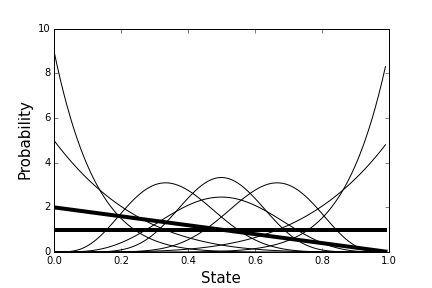
\includegraphics[width=\textwidth]{beta-distribution.png}
\caption{Beta distribution for various parameter values of $\alpha$ and $\beta$, including the uniform distribution $\alpha = \beta = 1$.}
\label{beta-distribution}
\end{figure}

\begin{table}
\begin{tabular}{@{}cccc|c@{}}
\hline
       &\textsc{discourse new} & \textsc{Inferrable} & \textsc{discourse old} & \textsc{total}\\
\hline
1150-1250    & 393  & 203 & 52   & 648  \\
1250-1350    & 346  & 296 & 42   & 684\\
1350-1420    & 294  & 179 & 60   & 533\\ \hline
\textsc{total} &1033 & 678 & 154 & 1865 \\
\end{tabular}
\caption{Distribution of sentence activation from \cite{wallage2013}}
\end{table}

\begin{itemize}
	\item $\chi$ test, show that we can collapse across time periods
	\item We can collapse across time periods to fit prior.
	\item What's a good fit of beta distribution? $\alpha = 1, \beta = 2$
	\item 
\end{itemize}

\section{Equilibria}

Determining the equilibria of the game we described will allow us to address several questions about how signals are used in the functional cycle. Broadly speaking, we want to know two things. First, we want to understand the relationship between senders' tendency to overestimate activation and the use of signals at equilibrium. In particular, we want to know how large this bias can be while still allowing for informative signaling. Second, we want to know whether particular equilibria constitute evolutionarily stable strategies. If so, we want to know the strategies that are evolutionarily stable. If not, we want to know what strategies could invade the population and disturb an equilibrium.

To answer these questions we first determine the equilibria of the game, which means we need the expected utility of sender and receiver strategies. Where the prior probability is given by the empirical distribution we determined in the last section, these are the following equations.

\begin{equation}
     E[U_S(s, r)] = \int \left( 1 -(r(s(t)) - t - (1-t)b)^2 \right)p(t)dt
\end{equation}

\begin{equation}
      E[U_R(s, r)] = \int \left( 1 -(r(s(t)) - t)^2 \right) p(t) dt
\end{equation}
These are exactly analogous to expected utility in the discrete case, where we summed over all the possible states. Again, $r(s(t))$ is the receiver's respond to the sender's message and yields an action, which determines the utility for both sender and receiver given a state.

The set of sender strategies is all potential mappings from the unit interval to a discrete set. This is a bit problematic given that the domain is uncountable. To simplify things we consider the following condensed representation. Let $\mathcal{P}_n(T)= t_0 = 0 < t_1 < ... < t_{n-1} < t_n = 1$ be a partition of the state space into $n$ subintervals.  For each properly defined subinterval, $(t_{i-1},t_i)$ the sender uses the message $m_i$. A speaker's strategy is then a function from this partition to messages $S : [\mathcal{P}_n(T) \rightarrow M]$.  Intuitively, this is simply a way of carving up the state space into discrete contiguous regions and using those regions to determine which signal to send. For example, consider the case of two messages $\mathcal{P}_2(T)$, where $m_1$ and $m_2$ correspond to \textcolor{red}{\emph{ne}} and \textcolor{blue}{\emph{ne...not}} respectively. For $t \in (0, t_1)$ a sender will use  \textcolor{red}{\emph{ne}} and for $t \in (t_1, 1)$ a sender will use \textcolor{blue}{\emph{ne...not}}.

The set of receiver strategies is all potential mappings from the set of messages to the unit interval. Since the domain is finite, this is more straightforward than the set of sender strategies. For each message $m_i$ the receiver takes an action $a_i$. So, for example, $a_1$ would be the receiver's response to message $m_1$, in this case \textcolor{red}{\emph{ne}}, and $a_2$ would be the receiver's response to message $m_2$, in this case \textcolor{blue}{\emph{ne...not}}.

Now that we have defined the set of sender and receiver strategies, we can ask what strategies constitute evolutionarily stable strategies. Given that signaling games are asymmetric, this amounts to identifying the strict Nash equilibria of the game. This can be done by determining what strategies jointly maximize the expected utilities of senders and receivers. Let $\langle s^*, r^* \rangle$ be an equilibrium strategy profile. In this case, $s^*((0, t_1^*)) = m_1$, $s^*((t_1^*, 1)) = m_1$, $r^*(m_1) = a_1^*$ and $r^*(m_2) = a_2^*$. We have two functions that we want to maximize with respect to three variables. To do so, we need to find the conditions where the following hold.

\begin{equation}
	\frac{\partial E[U_S(s, r)]}{\partial t_1^*} = 0
\end{equation}

\begin{equation}
	\frac{\partial E[U_R(s, r)]}{\partial a_1^*} = \frac{\partial E[U_R(s, r)]}{\partial a_2^*} = 0
\end{equation}
We can determine the equilibrium for two messages for any amount of bias, and this is shown in Figure \ref{sol2-beta}.\footnote{See Appendix A for code to calculate the full functional form of the solution.} Along the horizontal axis is the amount of sender bias, the vertical axis represents the point at which senders partition the state space and the actions of receivers. For any value of the sender bias $b$, the solid black line represents the point at which senders partition the state space $t_1^*$ and the dashed lines represent receiver responses to the different messages, $a_1^*$ and $a_2^*$.

\begin{figure}
	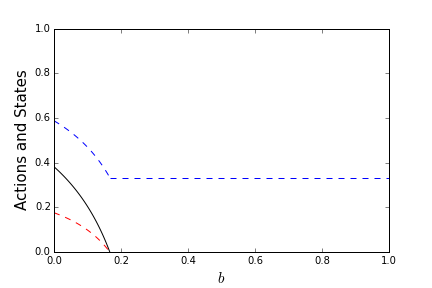
\includegraphics{sol2-beta.png}
	%
	\caption{Equilibrium solution for two messages for values of bias}
	\label{sol2-beta}
\end{figure}

There are several things to note about the equilibria solutions for two messages. First, the point at which senders partition the state space strictly decreases in the amount of bias. The more biased that senders are the more that senders will use message $m_2$. For $ b > \frac{1}{6}$ this is the only message that gets used in equilibrium, which is exactly what we see in Figure \ref{sol2-beta}. In fact, for any number of messages $n$ there exists a maximum amount of bias $b_n$ such that all messages are used in equilibrium. For any number of messages \cite{crawford-sobel:1982} show that $b_n > b_{n+1}$. That is, for a given number of messages, there is a maximum amount of bias that allows for all messages to be used in equilibrium. As speakers' bias decreases, $b \rightarrow 0$, the number of messages that can be used in equilibrium goes to infinity. This makes sense insofar as the closer the incentives of senders and receivers, the finer and more detailed the information senders want to signal. The number of messages available is the only limit on the amount of information conveyed when the interests of both parties are perfectly aligned.

Second, the receiver's best response to the different messages is the action that corresponds to the expected value of the portion of the partition that it corresponds to. That is, $a_1^* = E[t \mid t < t_1^*]$ and $a_2^* = E[t \mid t > t_1^*]$. These receiver responses are \emph{Bayes estimators}, the actions which maximize the utility function given the receipt of a signal.\footnote{Note that maximizing a utility function is the same as minimizing a loss function.} When sender bias is sufficiently large, and only one message is used in equilibrium, it carries no additional information about the sender's state. There is no information gained about the sender by receiving the signal, which is exactly why the Kullback-Leibler divergence between two distributions is also referred to as the \emph{information gain}.  For the continuous case, for a given signal we compare the prior distribution over states to the posterior distribution after hearing the signal.

\begin{equation}
     KL(m) = \int log\left( \frac{p(t \mid m)}{p(t)}  \right)p(t \mid m) dt
\end{equation}
If the posterior is the same as the prior, as is the case when a single message is used, then the information gained is zero. This follows directly from the definition of information gain, the logarithm of one is zero.

Interestingly this matches with Israel's \citeyearpar{israel2001} notion of informativity relative to some expected norm. That is, assume that there is some scalar \emph{norm} for how negation is to be used. In this case, this is simply the prior probability over states. A form of negation is informative relative to prior expectation if it picks out, or elicits a response that is  high in response to the scalar norm. For example, suppose that 

%For a given number of messages, we can calculate the maximum amount of bias for all of the messages to be used in equilibrium. That is, if the amount of bias exceeds a certain amount, then not all messages will be used in equilibrium. These constraints can be shown in Figure \ref{max-bias-uniform} where the number of messages is shown along the horizontal axis and the maximum amount of bias compatible with that number of messages to be used in equilibrium is shown along the vertical axis.

%\begin{figure}
%	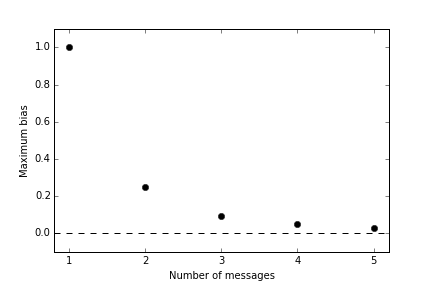
\includegraphics{max-bias.png}
%	%
%	\caption{Maximum value of $b$ that allows for a given number of messages in equilibrium.}
%	\label{max-bias-uniform}
%\end{figure}

%There are two things to be noted about the relationship between the amount sender bias and the number of messages used in equilibrium.  First, as the number of messages increases, the amount of bias must correspondingly decrease. Or, put differently, if we were to flip Figure \ref{max-bias-uniform} on its side, we might note that as sender bias decreases, the amount of potential messages  in equilibrium increases to infinity. That is, if senders had access to an uncountably infinite set of messages, then they could make an infinitely fine partition that would perfectly pick out the state. Second, there is a maximum amount of bias that allows for the transmission of any information. If $b > \frac{1}{4}$ then only one message is used in equilibrium. This means that the single message cannot carry any information since the signal cannot alter the prior beliefs of receivers. 



\section{Dynamics}

\section{Modeling}

\begin{figure}
\centering
     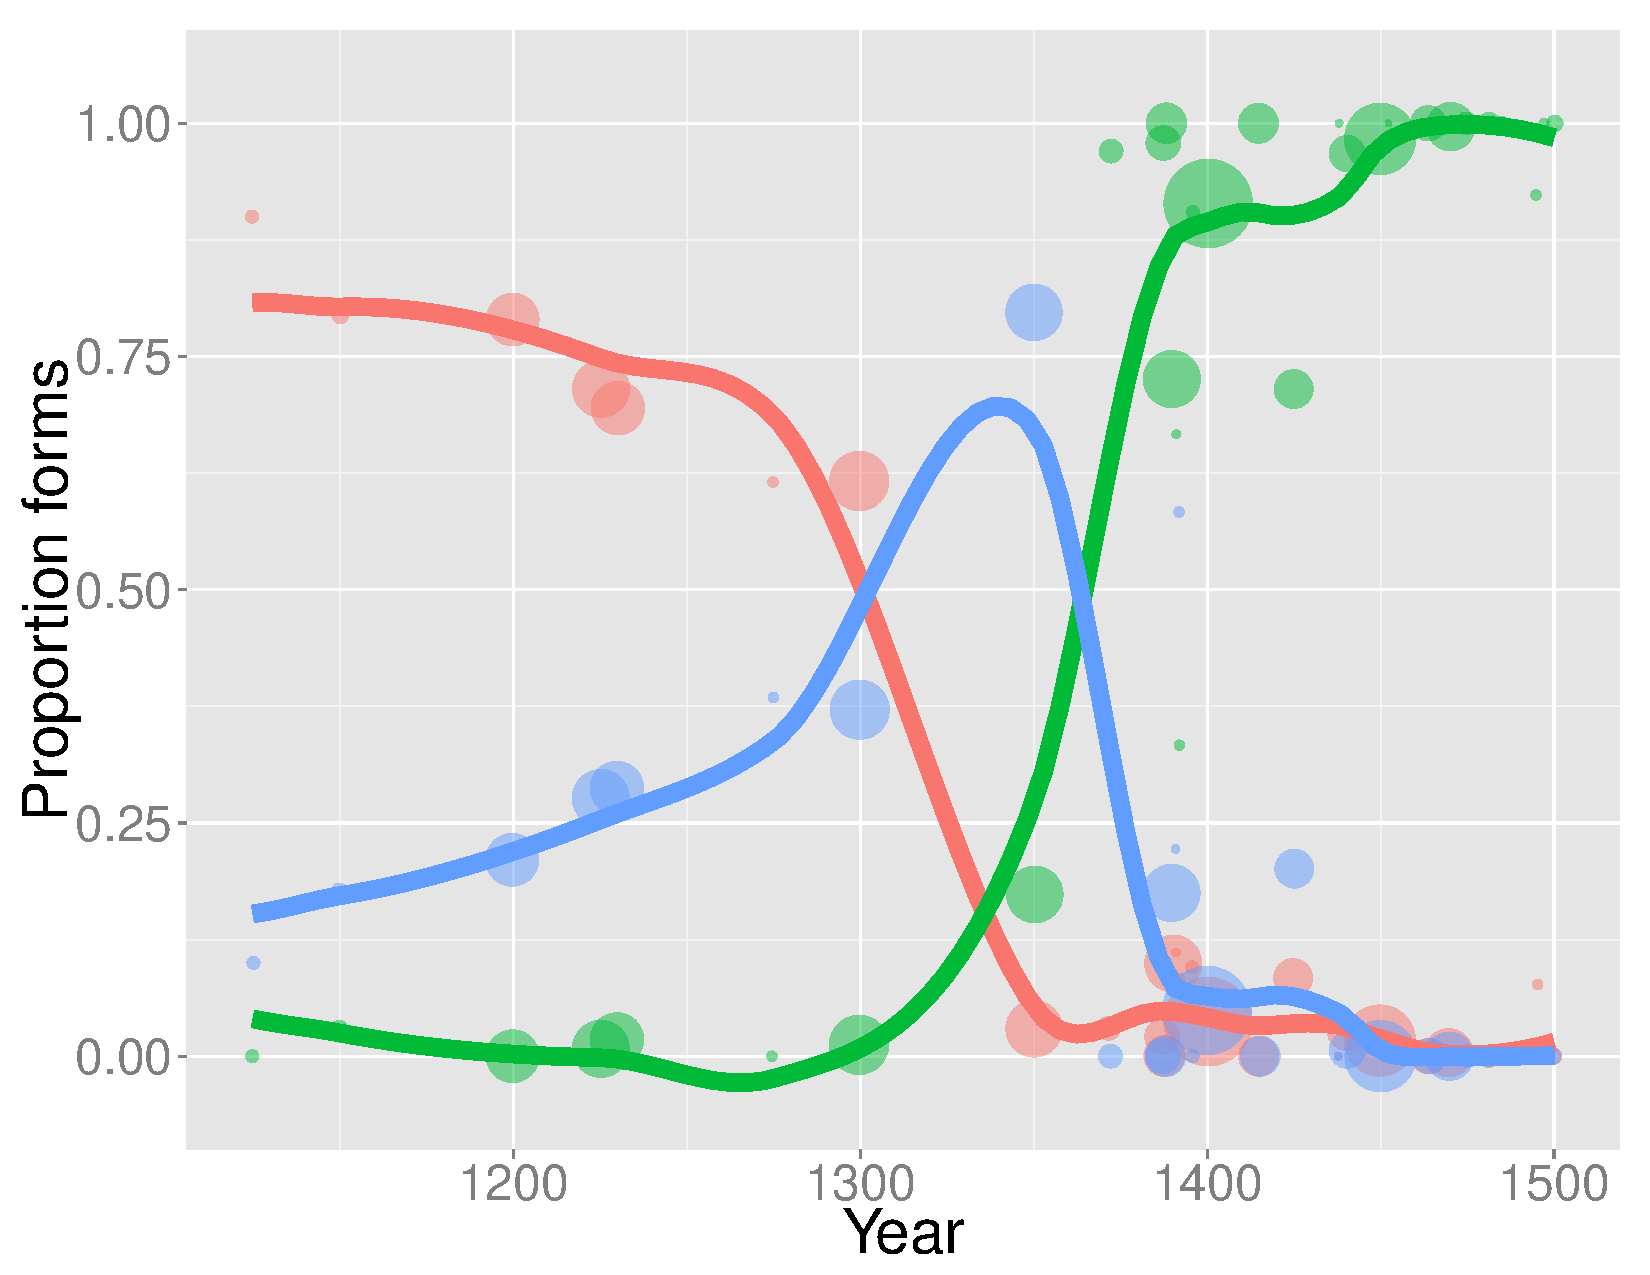
\includegraphics[width=\textwidth]{neg-year-lines.pdf}
\caption{Proportion of forms of negation in Negative Declaratives}
\label{neg-three-plot}
\end{figure}

\begin{figure}
\centering
     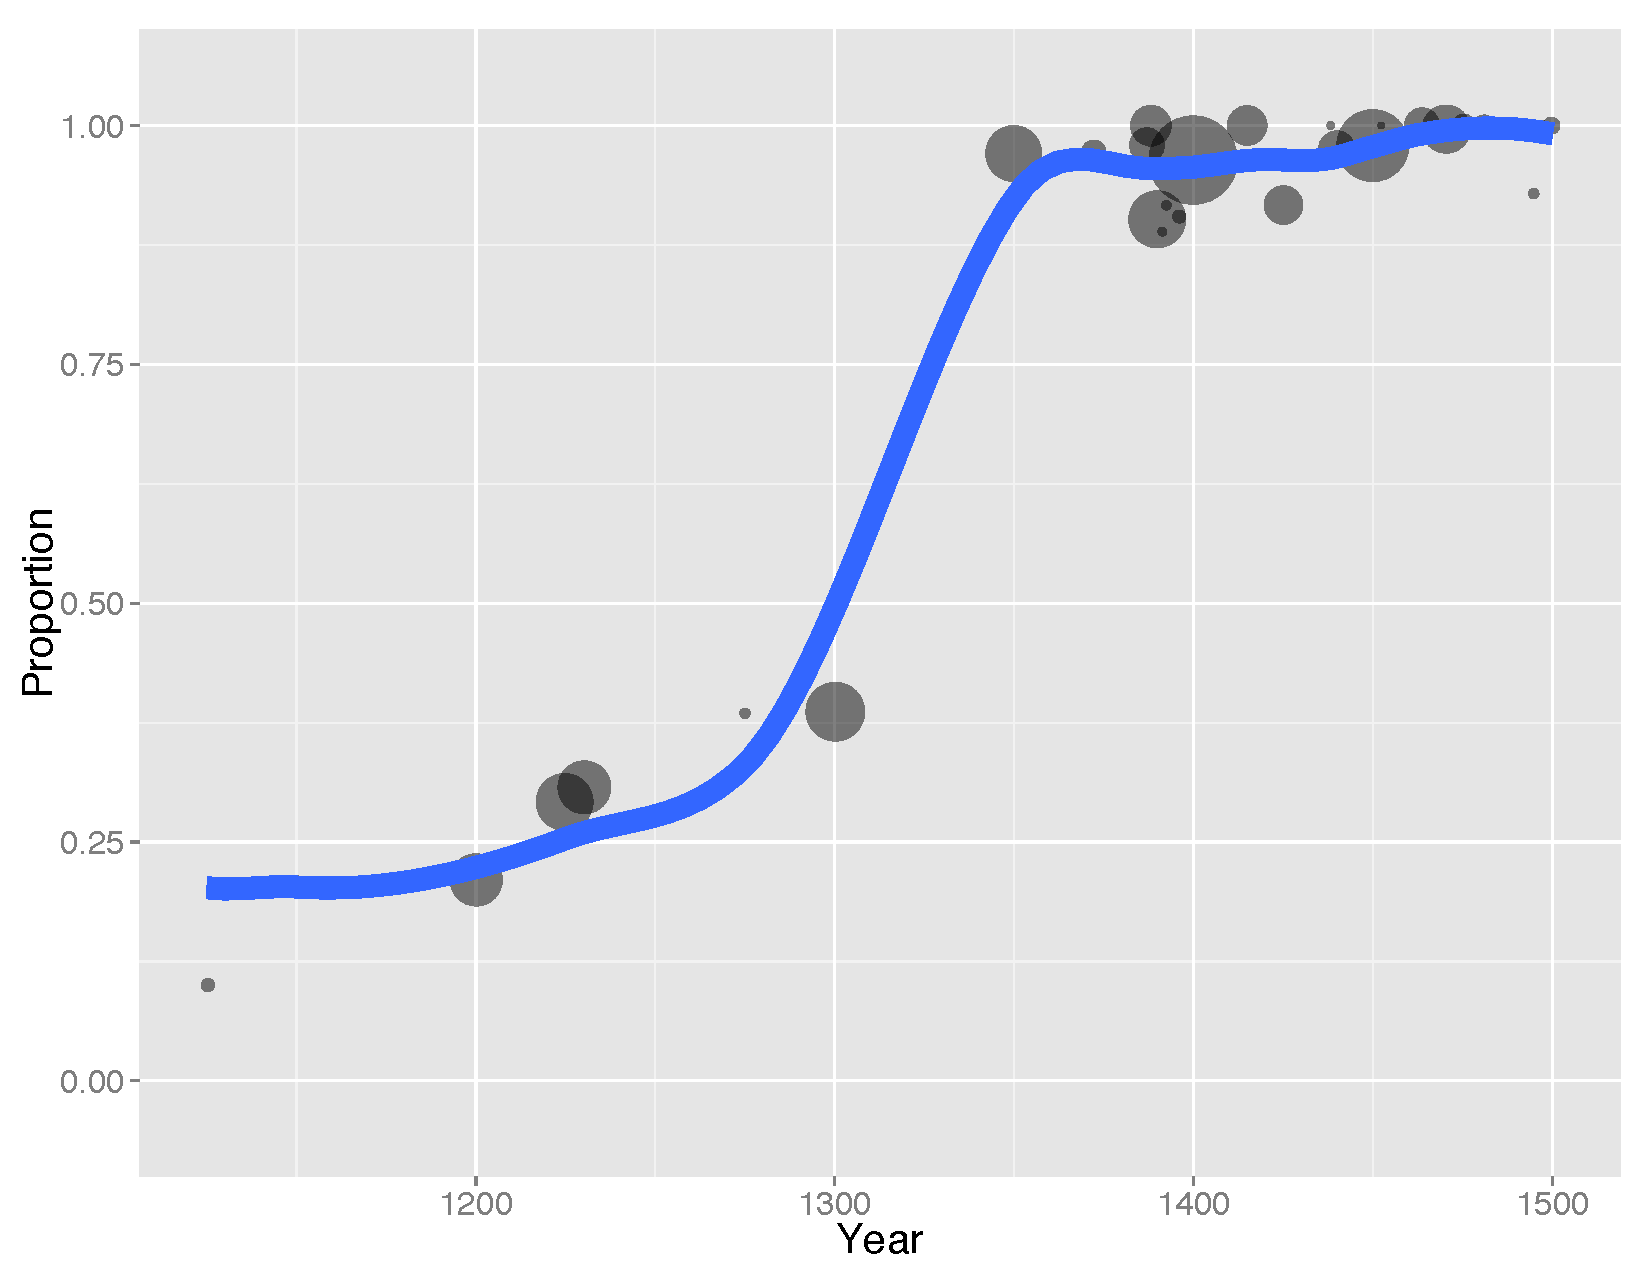
\includegraphics[width=\textwidth]{lump-plot1.pdf}
\caption{Proportion of \textit{\color{blue} ne...not} and \textit{\color{green} not}  versus  \textit{\color{red}  ne} over time}
\label{lump-plot1}
\end{figure}


\section{Summary}

givenness hierarchy

\begin{itemize}
	\item In focus, activated, familiar, unique, referential, type
	\item Old english : demonstrative to definite
	\item Different prior distribution 
\end{itemize}



% Bibliography
\bibliographystyle{mcbride}
\bibliography{ahern}

\end{document}